\documentclass[11pt, a4paper]{article}
\title{Wacky Racers 2020 Instructions}
\author{Michael Hayes, Ben Mitchell}
\date{Version 2, \today}

\usepackage[margin=1in]{geometry}
\usepackage{parskip}
\usepackage{float}
\usepackage{todonotes}
\presetkeys{todonotes}{inline}{}
\usepackage{graphicx}
\usepackage[T1]{fontenc}
\usepackage{makecell}
\usepackage[breaklinks=true]{hyperref}
\usepackage{tabularx}
\usepackage{subcaption}
\usepackage{listings}
\usetikzlibrary{arrows}

\newcommand{\code}[1]{\texttt{#1}}


\begin{document}
\maketitle

\section{Introduction}

The purpose of this assignment is to design, build, and program an
embedded system using an ARM microcontroller and surface mount
technology.

The goal for each group of four students is to build a remote
controlled vehicle (the Wacky Racer) and its controller (the Wacky
Hat).  At the conclusion of the assignment there will be a dastardly race!

Each group is comprised of two sub-groups of two students.  One of
these subgroups constructs the Wacky Racer and the other constructs
the Wacky Hat.  You may be asking why is the Wacky Hat called the
Wacky Hat?  Well, a hat that controls a remote vehicle using head
motions is not an ordinary hat!


\section{Requirements}

The following requirements are mandatory if you wish to maximise your
marks.


\subsection{Wacky racer}

\begin{enumerate}
\item The chassis is to be constructed by each group.  These can be
  3-D printed, constructed from Perspex or wood, etc.  A standard
  chassis is available from the Automation Lab technician (Daniel
  Hopkins).  The electronics must be visible on top of the chassis.
\item Have a standard working bump sensor (supplied).  
\item Locomotion can only use two 6\,V DC motors (supplied).
\item Everything must be powered from a single 6-cell NiMH battery pack (supplied).
\item Use a single four layer printed circuit board of dimension 85\,mm$\times$64\,mm.
\item Use an ARM microcontroller (Atmel SAM4S8).
\item Drive the motors using H-bridges (Texas Instruments DRV8833 dual
  H-bridge is recommended).
\item Regulate the nominal battery voltage to 5\,V with a buck
  regulator IC (ADP2302ARDZ-50).
\item Be decorated with an LED tape (supplied) controlled by the MCU.
\item Use a USB interface for debugging.
\item Use a serial wire debug interface for MCU programming/debugging.
\item Have adequate battery fusing and reverse polarity protection.
\item Have a sleep button.
\item If the battery voltage drops below 1\,V/cell, an LED should flash and high power draw devices should be disabled.
\item Interface to the Wacky Hat with a Nordic nRF24 SMD radio module.
\item Have four jumper selectable radio channels.  
\item Have a mounted RFID card (supplied) that can be read by the Wacky ramps.
\item Be humorous.    
\end{enumerate}


Each Wacky Racer can have a dastardly means of hindering another
team's Wacky Racer.  However, you cannot:
%
\begin{itemize}
\item Damage or destroy another Wacky racer
\item Damage the venue
\item Injure a spectator
\item Jam the radio signals  
\end{itemize}


\vspace{1cm}

\begin{figure}[h]
    \centering
    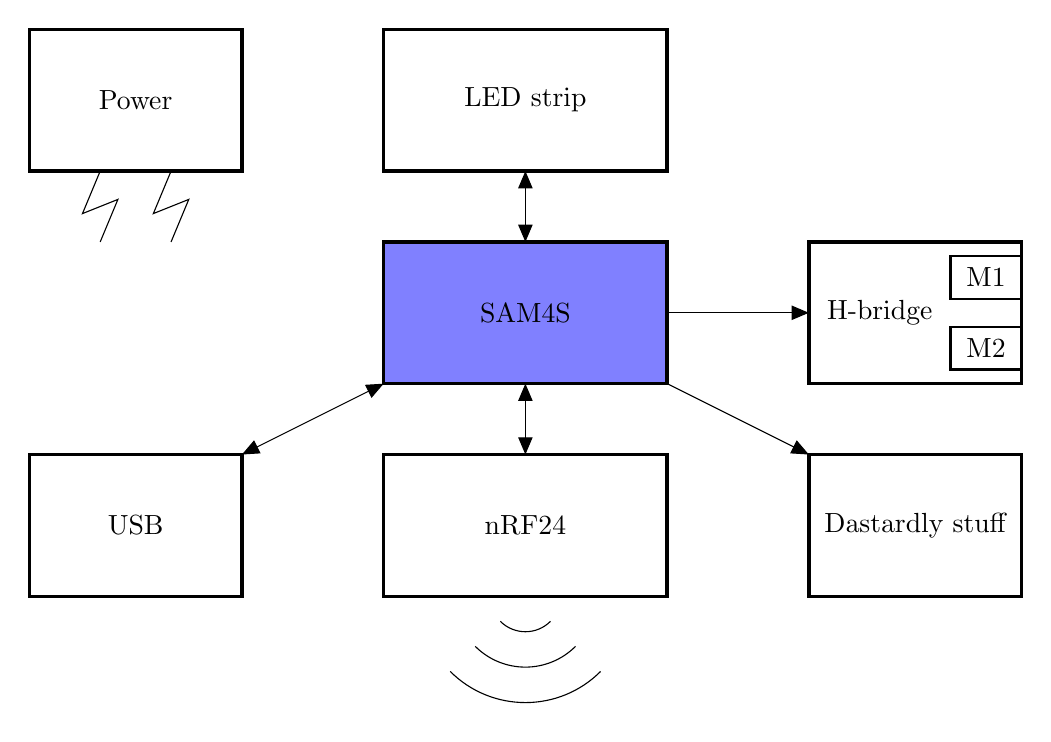
\begin{tikzpicture}[scale=0.9]
    
    \draw[black, very thick, fill=blue!50] (-2, -1) rectangle (2, 1);
    \node at (0, 0) {SAM4S};

    % H-bridge
    \draw[black, very thick] (4, -1) rectangle (7, 1);
    \node at (5, 0) {H-bridge};
    \draw[-triangle 45] (2, 0) -- (4, 0);
    \draw[black, thick] (6, 0.8) rectangle (7, 0.2);
    \node at (6.5, 0.5) {M1};
    \draw[black, thick] (6, -0.8) rectangle (7, -0.2);
    \node at (6.5, -0.5) {M2};
    

    % Dastardly
    \draw[black, very thick] (4, -2) rectangle (7, -4);
    \node at (5.5, -3) {Dastardly stuff};
    \draw[-triangle 45] (2, -1) -- (4, -2);

    % LED strip
    \draw[black, very thick] (-2, 2) rectangle (2, 4);
    \node at (0, 3) {LED strip};
    \draw[triangle 45-triangle 45] (0, 1) -- (0, 2);

    % Radio
    \draw[black, very thick] (-2, -2) rectangle (2, -4);
    \node at (0, -3) {nRF24};
    \draw[triangle 45-triangle 45] (0, -1) -- (0, -2);
    \draw (0.354, -4.354) arc (-45:-135:0.5);
    \draw (0.707, -4.707) arc (-45:-135:1);
    \draw (1.061, -5.061) arc (-45:-135:1.5);

    % Power
    \draw[black, very thick] (-4, 2) rectangle (-7, 4);
    \node at (-5.5, 3) {Power};
    \draw (-5, 2) -- (-5.25, 1.4) -- (-4.75, 1.6) -- (-5, 1);
    \draw (-6, 2) -- (-6.25, 1.4) -- (-5.75, 1.6) -- (-6, 1);
    
    % USB
    \draw[black, very thick] (-4, -2) rectangle (-7, -4);
    \node at (-5.5, -3) {USB};
    \draw[triangle 45-triangle 45] (-2, -1) -- (-4, -2);

    
\end{tikzpicture}

    \caption{Racer board top level diagram.}
\end{figure}


\vfill\pagebreak

\subsection{Wacky hat}


\begin{enumerate}
\item Construct a Wacky Hat that contains all the electronics.
\item Everything must be powered from a single 6-cell NiMH battery pack (supplied).  
\item Have adequate battery fusing and reverse polarity protection.
\item Use a single four layer printed circuit board of dimension 85\,mm$\times$64\,mm.  
\item Use an ARM microcontroller (Atmel SAM4S8).
\item Regulate the nominal 6\,V battery voltage to 5\,V with a buck
  regulator IC (ADP2302ARDZ-50).
\item Be decorated with an LED tape (supplied) controlled by the MCU.
\item Use an I2C IMU (MPU-9250) for head motion detection.
\item Use a USB interface for debugging.
\item Use a serial wire debug interface for MCU programming/debugging.
\item Have a joystick in case the IMU does not work.
\item Have a sleep button.
\item If the battery voltage drops below 1\,V/cell, an LED should flash and high power draw devices should be disabled.
\item Play sound when the bumper is hit.
\item Interface to the Wacky Racer with a Nordic nRF24 SMD radio module.  
\item Have four jumper selectable radio channels.    
\item Be humorous.  
\end{enumerate}

%\vspace{1cm}

\begin{figure}[h]
  \centering
  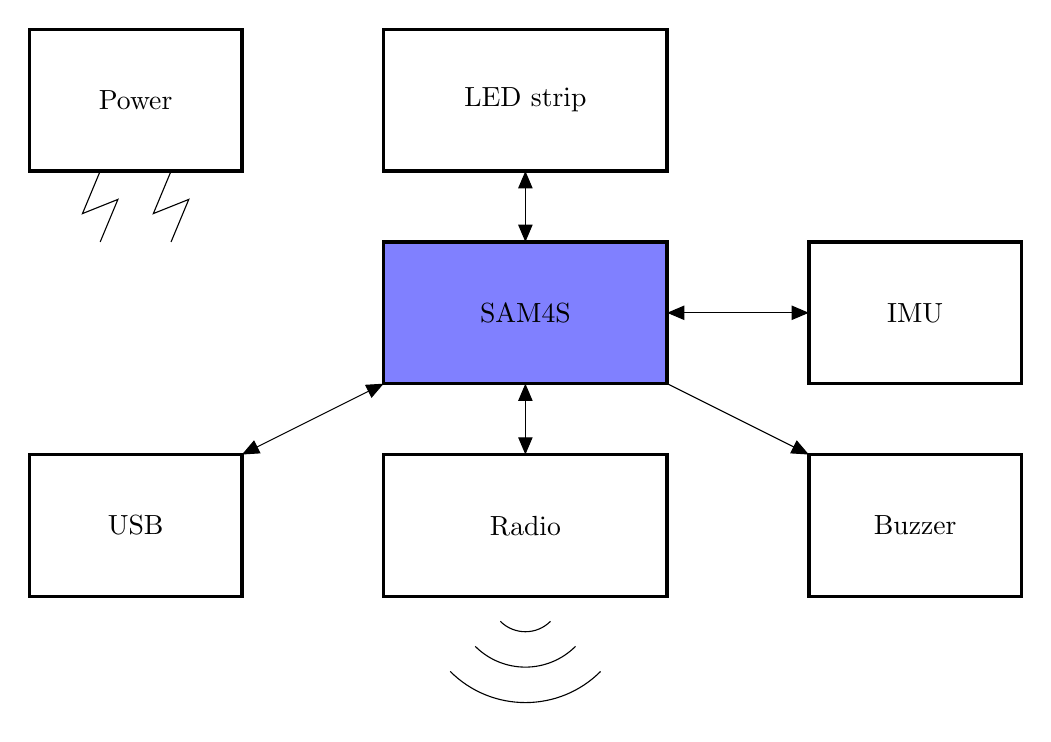
\begin{tikzpicture}[scale=0.9]
    
  \draw[black, very thick, fill=blue!50] (-2, -1) rectangle (2, 1);
    \node at (0, 0) {SAM4S};  

    % IMU
    \draw[black, very thick] (4, -1) rectangle (7, 1);
    \node at (5.5, 0) {IMU};
    \draw[triangle 45-triangle 45] (2, 0) -- (4, 0);

    % Buzzer
    \draw[black, very thick] (4, -2) rectangle (7, -4);
    \node at (5.5, -3) {Buzzer};
    \draw[-triangle 45] (2, -1) -- (4, -2);

    % LED strip
    \draw[black, very thick] (-2, 2) rectangle (2, 4);
    \node at (0, 3) {LED strip};
    \draw[triangle 45-triangle 45] (0, 1) -- (0, 2);

    % Radio
    \draw[black, very thick] (-2, -2) rectangle (2, -4);
    \node at (0, -3) {Radio};
    \draw[triangle 45-triangle 45] (0, -1) -- (0, -2);
    \draw (0.354, -4.354) arc (-45:-135:0.5);
    \draw (0.707, -4.707) arc (-45:-135:1);
    \draw (1.061, -5.061) arc (-45:-135:1.5);

    % Power
    \draw[black, very thick] (-4, 2) rectangle (-7, 4);
    \node at (-5.5, 3) {Power};
    \draw (-5, 2) -- (-5.25, 1.4) -- (-4.75, 1.6) -- (-5, 1);
    \draw (-6, 2) -- (-6.25, 1.4) -- (-5.75, 1.6) -- (-6, 1);
    
    % USB
    \draw[black, very thick] (-4, -2) rectangle (-7, -4);
    \node at (-5.5, -3) {USB};
    \draw[triangle 45-triangle 45] (-2, -1) -- (-4, -2);

    
\end{tikzpicture}

  \caption{Racer hat top level diagram.}
\end{figure}


\pagebreak

\section{Assignment schedule}

There is a planned activity for the timetabled labs in the Embedded
Systems Lab (ESL):
%
\begin{flushleft}
  \begin{tabular}{ c l l }
    Week            &  Assistance  &  Assessment \\
    \hline \hline
    T1-1 & Altium tutorial 1 (schematics)  & \\
    T1-2 & Altium help       & \\
    T1-3 & Schematic review  &  Schematic submission for review (Mon. noon) \\
    T1-4 & Altium tutorial 2 (PCB) &          \\
    T1-5 & Altium help & PCB submission 1    \\
    T1-6 & Altium help & PCB submission 2    \\
    T1-7 & General     & PCB submission 3    \\ \hline
    B-1 & (break)    &                   \\
    B-2 & (break)    &                   \\
    B-3 & (break)    &                   \\ \hline
    T2-1 & General     & Blinky            \\
    T2-2 & General     & IMU/motors      \\
    T2-3 & General     & Radio control     \\    
    T2-4 & General     & Functionality     \\
    T2-5 & Competition & Competition, critique  \\
  \end{tabular}
\end{flushleft}


Notes:
%
\begin{enumerate}
\item There there may be a 6--10 day delay for the PCBs to be
  manufactured from the time of submission.  You will then need to
  book an assembly session in the SMT lab provided you have done the
  SMT lab induction.

\item Do not underestimate the blinky milestone.  It requires having a
  functional PCB with a microcontroller that turns on properly, a
  functional toolchain and the ability to download code into the
  microcontroller's flash memory.
\end{enumerate}


\section{Assessment}

The marks breakdown (max. 0x64) is:
%
\begin{flushleft}
  \begin{tabular}{ll}
    PCB submission & 0--0xa marks\\
    Blinky milestone  & 0x5 marks\\    
    IMU/motor milestone  & 0x5 marks\\
    Radio control milestone  & 0x5 marks\\
    Functional assessment & 0--0x14 marks \\
    Board inspection & 0--0x1e marks \\
    Competition & 0--0xa marks \\
    Individual critique & 0--0xf marks \\
  \end{tabular}
  
\end{flushleft}

\subsection{Milestones}

There are five milestones.  To achieve the associated marks, they must
be demonstrated to a T.A. by the end of the lab for your allotted
stream.  If you need an exception to this, see Ben Mitchell with a
\emph{very} good reason.  The milestone requirements are:
%
\begin{description}
\item [Schematic review] Submit your A3 schematic on Learn for
  review.  Lose 10 marks if you miss the submission time.

\item [PCB submission] Submit your PCB design to Learn for
  manufacture.  To encourage early submission there is a sliding scale
  for marks depending on when the PCB is submitted, see table.  After
  week 7, there is a 10 mark penalty per week.  \textbf{NB, a rushed
    PCB design will cause you more grief, more PCB rework, and a lower
    mark for the inspection.}

  \begin{tabular}{llll}
    Week & Submission day & Cut-off time  & Mark \\ \hline
    5    & Monday       & 10.00 am & 10 \\
    5    & Wednesday    & 10.00 am & 9 \\
    5    & Friday       & 10.00 am & 8 \\
    6    & Monday       & 10.00 am & 7 \\
    6    & Wednesday    & 10.00 am & 6 \\
    6    & Friday       & 10.00 am & 5  \\
    7    & Monday       & 10.00 am & 4 \\
    7    & Wednesday    & 10.00 am & 2 \\
    7    & Friday       & 10.00 am & 0 \\        
  \end{tabular}

\item [Blinky] Demonstrate that can blink an LED controlled by the SAM4S.
  
\item [IMU/motors] For the Wacky Hat, demonstrate output of IMU
  readings to a PC using USB CDC.  For the Wacky Racer, demonstrate
  control of the motors from a PC using USB CDC.

\item[Radio control] Demonstrate sending commands from the Wacky Hat
  to the Wacky Racer over a radio link.
\end{description}

\textbf{If you cannot show the functionality of a previous milestone
  during any assessment, you will fail that assessment and loose any
  marks from the previous milestone.}


\subsection{Functionality assessment}

Functionality requirements:
%
\begin{flushleft}
  \begin{tabular}{l|l}
    Wacky racer & Wacky hat \\ \hline \hline
    Blink LED                      & Blink LED \\
    Drive motors forward/backward  & Read from IMU \\
    Speed control of motors        & Calculate speeds from IMU \\
    Steering control               & Joystick control \\
    Receive radio message          & Send radio message \\
    Jumper selectable radio channel & Jumper selectable radio channel  \\    
    Dies on bump                   & Plays sound on bump \\
    Report group info to game server & Report group info to game server \\
    Low voltage indication         & Low voltage indication \\
  \end{tabular}
\end{flushleft}
%
Marks are allocated on how well things work.  Up to 5 bonus marks can
be awarded for extra functionality such as:
%
\begin{flushleft}
  \begin{tabular}{l|l}
    Wacky racer                & Wacky hat \\ \hline \hline
    Dastardly stuff            & Plays interesting sounds \\
    Sleep mode                 & Sleep mode \\
  \end{tabular}
\end{flushleft}


\subsection{Competition}

The competition is a race around an obstacle course.  Marks will be
awarded every time you pass over a Wacky Ramp in the correct order.
These ramps have an RFID card reader that will detect your Racer if
you have correctly fitted an RFID card.  The Wacky Ramps change colour
when they detect a Wacky Racer.

To be awarded any marks for the race:
%
\begin{enumerate}
\item Your vehicle must stop for at least 5\,s if the bumper is hit.

\item Your vehicle must be controlled by motions of the Wacky hat
  sitting on someone's head.
\end{enumerate}


\subsection{PCB inspection}

This is assessed after the competition.  The categories are:
%
\begin{enumerate}
\item Layout (component placement etc.)
\item Construction (tidiness, rework, etc.)
\item Testability  
\item Power supplies (routing, decoupling, etc.)
\end{enumerate}



\section{Technical stuff}

Read this section carefully.  There are clues as to how we mark your
PCBs at the end of the assignment.


\subsection{Version control}

Use version control for everything, or else!  Learning git is
frustrating but is a skill you will not regret.

Your group leader should create a forked copy of the wacky-racers-2020
git project and then add the other group members to the project.  This
can be done by:

\begin{enumerate}
\item Go to \url{https://eng-git.canterbury.ac.nz/wacky-racers/wacky-racers-2020}

\item Click `Fork' button.  This will create a copy of the main repository for the project.

\item Click on the `Settings' menu then click the `Expand' button for
`Sharing and permissions'.  Change `Project Visibility' to `Private'.

\item Click on the `Members' menu and add group members as Developers.

\item Using a bash terminal (or other useful shell), enter the command:

  \lstset{language=bash}
  \lstset{basicstyle=\ttfamily\small}
  \lstset{keywordstyle=\color{black}\ttfamily}
  \lstset{breaklines}
  
\begin{lstlisting}
  $ git clone https://eng-git.canterbury.ac.nz/your-userid/wacky-racers-2020.git wacky-racers
\end{lstlisting}

If you do not want to have to enter your password for every git
push/pull operation, you should set up ssh-keys and use:

\begin{lstlisting}[breaklines]
  $ git clone git@eng-git.canterbury.ac.nz:your-userid/wacky-racers-2020.git wacky-racers
\end{lstlisting}

\item Add a remote URL for the main repository.
%
\begin{lstlisting}[breaklines]
  $ cd wacky-racers 
  $ git remote add upstream https://eng-git.canterbury.ac.nz/wacky-racers/wacky-racers-2020.git  
\end{lstlisting}
%
Again if you do not want to manually enter your password, you can use:
%
\begin{lstlisting}[breaklines]
  $ cd wacky-racers 
  $ git remote add upstream git@eng-git.canterbury.ac.nz:wacky-racers/wacky-racers-2020.git    
\end{lstlisting}
%
If we add more demo code or tweak the instructions in the main
repository, you can get the updated stuff using:
%
\begin{lstlisting}[breaklines]
  $ git pull upstream master
\end{lstlisting}
\end{enumerate}


\subsection{Components}

\begin{enumerate}
\item We recommend that you use components in the ECE Altium library.
  These are stocked in the SMT lab.  For any other components you may
  require, see Scott Lloyd in the SMT lab.

\item The Wacky Racer batteries are 6-cell NiMH with a three pin
  connector.  To preserve the battery life it is imperative to not
  draw current when the battery voltage is below 6\,V.
\end{enumerate}


\subsection{Connectors}

\begin{enumerate}
\item USB micro or mini connector for debugging
\item 3 pin 0.1'' for LED strip (pin 1 5\,V, pin 2 signal, pin 3 ground)
\item 2 pin 0.1'' for bumper (pin 1 switch, pin 2 ground)
\item 10 pin IDE for serial wire debug  
\item 3 pin power connector (pin 1 VBAT, pin 2 GND, pin 3 N.C.)
\item motor connectors (for Racer)
\item connectors for dastardly stuff
\end{enumerate}


\subsection{Schematics}

\begin{enumerate}
\item Have a look at the
  \href{http://ecewiki.elec.canterbury.ac.nz/mediawiki/index.php/ENCE461_Altium_tutorial}{Altium
    tutorial on ecewiki}.

\item Have a read of the
  \href{http://ecewiki.elec.canterbury.ac.nz/mediawiki/index.php/Schematic_guidelines}{schematic
    guidelines on ecewiki}.

\item Add you and your partner's name and your group number to the
  title block on your schematic.

\item Save PDF files of your schematics in your source repository.
  \textbf{Note, when debugging your PCBs, we will not help you until
    you show us your printed A3 schematic}.

\item We bet that you will not have enough test points to clip an
  oscilloscope probe to.  Do not think you can hold the probe tip
  against an MCU pin.  Ensure you give a meaningful name to the test
  point.  A ground test point is essential for an oscilloscope earth
  clip. Keep this clear of other test points since the clip may short
  against them.  You will probably require at least two ground points.
  
\item Checking the schematic is the most crucial part of the
  assignment.  If the schematic is wrong then your PCB will be wrong.
  So, schematics must be thoroughly checked by another person.

\item Consider fall-back options if you have a problem with your PCB.

  The IMU for the Wacky Hat is tiny and we \textbf{strongly recommend} that you
  provide an alternative connector for connecting the following IMU module:
  \href{https://www.aliexpress.com/item/SPI-IIC-MPU9250-MPU-9250-MPU-9250-9-Axis-Attitude-Gyro-Accelerator-Magnetometer-Sensor-Module-MPU9250/32216818498.html?spm=a2g0s.9042311.0.0.WKvtEm}{MPU-9250 on AliExpress}

  Similarly for the Wacky Hat, in case the H-bridge fails, provide two
  three-pin servo connectors so that external Electronic Speed
  Controllers (ESC) can be used to drive the motors.

\item It would be useful to have a jumper or two connected to a PIO
  pin so that you can configure your board.  For example, if a jumper
  is in, use the joystick, otherwise use the IMU.
  
\end{enumerate}


\subsection{PCBs}

\begin{enumerate}
\item Your four-layer PCBs are going to be manufactured in batches.
  There is at least a week turnaround time to get the boards made.

\item It is important that you check footprints for parts they you
  create.  We will impose a 10\% penalty for each rerun of a PCB, say
  due to a footprint mistake.  Get your partner to check.
  
\item PCB layouts must be thoroughly checked by another person.
  
\item A PCB track can blow faster than a fuse. So keep high current
  tracks fat and short.

\item Clearly mark the positive and negative battery connections on
  the silk screen.

\item Some of the chips can get hot so thermal considerations are
  required.  Follow the manufacturers' guidelines in the datasheets.

\item The switching regulators can interfere with the radios.
  
\item Use a design rule check to see if any of the following
  constraints are violated:
%
\begin{itemize}
\item Minimum trace width (0.15\,mm)
\item Minimum trace clearance (0.15\,mm)
\item Minimum via size (0.3\,mm hole, 0.6\,mm outer diameter)
\item Minimum hole size (0.3\,mm)
\item Minimum annular ring (0.1\,mm)
\end{itemize}
%
For every violation of one these rules, we will deduct 1\% from your
final mark.

\item Check the
  \href{http://ecewiki.elec.canterbury.ac.nz/mediawiki/index.php/PCB_checklist}{PCB
    checklist on ecewiki} before submission.
\end{enumerate}


\subsection{Assembly}

\begin{enumerate}
\item Finding shorts is extremely frustrating so maximise clearances
  and test for shorts before populating components.

\item Components can be put through the oven on the reverse side
  although heavy components may need to be glued.
  
\item Never assume where pin 1 is on an IC; check the datasheet.
  5--10\% of groups will get this wrong.
  
\end{enumerate}


\subsection{Software}

\begin{enumerate}
\item We highly recommend using a personal laptop with Linux installed if
possible. A virtual machine running on Windows is acceptable for this. You will
need to check instructions on ecewiki for how to install the required toolchain.

\item We do not support embedded systems development on Windows, but
  it is possible.

\item If you are not using version control for this you are foolish.

\item Inspect MPH's sample code.

\end{enumerate}


\subsection{Programming}

\begin{enumerate}
\item If you are trying to program the SAM4S for the first time and
  are feeling tired or impatient, then do something else.

\item For the first program, do not use batteries or a USB connection.
  The ST-Link adapter will provide 3.3\,V to the MCU.
 
\item Detailed instructions can be found at
  \url{http://ecewiki.elec.canterbury.ac.nz/mediawiki/index.php/Wacky_racers_software}.
\end{enumerate}


\subsection{Debugging}

\begin{enumerate}
\item Start running small programs (such as the provided demo
  programs) to test each feature separately.
  
\item An oscilloscope is your friend.

\item It is possible to use the GDB debugger but you need to know what
  you are doing, especially with optimised code.

\item Drawing a diagram of what you think is happening is highly recommended. A
simple circuit diagram or timing diagram will often help you realise what you
have missed and let you fix it without asking for help.
  
\end{enumerate}


\subsection{Possibly asked questions with answers}

\begin{itemize}
\item \emph{Why use the SAM4s MCU?}  For this application most MCUs
  would suffice, even an 8-bit AVR microcontroller.  To level the
  playing field, I have chosen a MCU most students would not have used
  before.  This is an ARM based MCU made by Atmel I have used this in
  a number of projects.  Indeed we used to teach this chip in ENCE361.
  There are many other similar MCUs made by different manufacturers
  such as the STM32 that would just as suitable.

\item \emph{Why use a four layer PCB?}  Come to lectures to find out!

\item \emph{Why use 7.2\,V NiMH batteries for the Wacky Racers?}
  These were a legacy of previous Wacky Racers.  They are also safer
  than lithium batteries with sleep-deprived students.

%% \item \emph{Why can't I program my device using Windows?} Due to
%%   various aspects of the Windows ecosystem, setting up a fully
%%   functional build environment is more complicated, will often vary
%%   from machine to machine, will often break filepaths, and will often
%%   cause bizarre compilation errors. Use at your own risk, we will not
%%   assist in debugging issues related to Windows.

\end{itemize}


\section{Assistance}


\begin{itemize}
\item Emails to the lecturers (except of a personal nature) will be
  quietly ignored.

\item Questions anwered on the ENCE461 Learn discussion page will be
  promptly answered.

\item All decisions regarding legality of your dastardly devices are
  at the whim of Ben Mitchell.  You can email Ben at
  \url{mailto://ben.mitchell@pg.canterbury.ac.nz} if you wish to keep
  your ideas secret.

\item TAs will be available in the scheduled lab times.  Priority will
  be given to groups assigned to the current lab session.  We will
  only provide assistance to students who have a printed A3 schematic
  sheet in front of them and have already tried looking up the problem
  on \url{https://ecewiki.elec.canterbury.ac.nz}.

\item Questions pertaining to Altium and surface mount rework will be
  answered by Scott Lloyd (SMT Lab technician) and Diego Ramirez
  (Electronics Lab technician).

\item Michael Hayes is really busy pulling all the string behind the
  scenes and so will only help with gnarly problems referred to by the
  TAs!
  
\end{itemize}

\end{document}
